
%(BEGIN_QUESTION)
% Copyright 2007, Tony R. Kuphaldt, released under the Creative Commons Attribution License (v 1.0)
% This means you may do almost anything with this work of mine, so long as you give me proper credit

The following illustration shows a rather strange manometer, one with two different liquids inside, coupled by a hand valve:

$$\includegraphics[height=7cm]{i02952x01.eps}$$

If the two columns of liquid are just right, they will remain at their respective (different) heights when the valve is opened.  Unlike a normal manometer where the two liquid columns always equalize to the same height when vented, this manometer is ``content'' to rest at different heights.  Explain why.

\vskip 10pt

Also, calculate two possible heights that will balance each other, given the liquids of water and glycerine.

\underbar{file i02952}
%(END_QUESTION)





%(BEGIN_ANSWER)

19 inches of water and 15 inches of glycerine will balance one another in this manometer.  These are not the only column heights that will self-balance.  In fact, any ratio of 19:15 will work because the ratio of water's density to glycerine's density is 15:19.

%(END_ANSWER)





%(BEGIN_NOTES)

%INDEX% Physics, static fluids: hydrostatic pressure

%(END_NOTES)


